%% Local IspellDict: brasileiro

\documentclass[11pt]{article}
\usepackage{relatorio-pibic}
\usepackage[utf8x]{inputenc}
\usepackage{cite}
\usepackage{subfig}

% usar para palavras estrangeiras: \eng{english word}
\newcommand{\eng}[1]{\textit{#1}}

\begin{document}

\graphicspath{{figs/}}

\cabecalho{Relatório Final}

\dadosRelatorioFinal
{Levantamento de operações de teorias de contornos em análises de
  obras musicais}
{Verificando inconsistências nas teorias de contornos musicais através
  de ferramentas computacionais }
{Eduardo Lago Nunes}
{Marcos da Silva Sampaio}
{Genos}
{Teoria de Relações de Contornos Musicais, Teoria Musical, Computação Musical}
{JANEIRO A JULHO DE 2012}

\resumo{Inserir texto do resumo}

\newpage

\setcounter{page}{1}
\onehalfspace

\Section{Introdução}
\label{sec:introducao}
\info{Delimitação do problema trabalhado e as conexões entre o plano
  de trabalho do bolsista e o projeto do orientador. Objetivos e
  justificativa do plano em termos de relevância para a pesquisa
  cientifica e do estado da arte.}
% importância de contornos para música, da teoria de contornos, a
% inconsistência...

Contorno é uma linha que marca externamente uma figura ou um objeto, uma espécie
de perímetro, caminho que cerca o redor de algum lugar ou algo. Em música pode-se
visualizar o contorno de diversos aspectos como altura, densidade, ritmo, timbre, etc.
\cite[p. 01]{Sampaio2008}.

\begin{figure}
  \centering
  \subfloat[Melodia]{
    \includegraphics{melodia}
    \label{fig:melodia}
  }
  \subfloat[Contorno < 3 0 1 4 2 >]{
    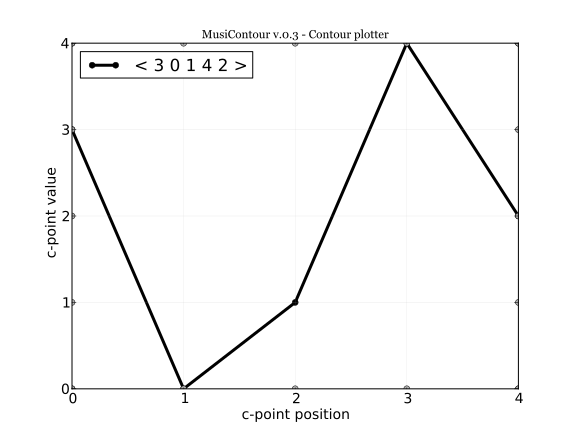
\includegraphics[scale=.3]{30142}
    \label{fig:30142}
  }
  \caption{Melodia e representação do contorno de alturas}
  \label{fig:melodia-representacao}
\end{figure}

% Marcos: reescrever
% Eduardo: Ok.
% Marcos: Clifford: aspecto estrutural em webern
% Marcos: ver análises de obras com enfoque nos contornos
Contornos são importantes por serem mais perceptíveis que notas 
até mesmo para ouvintes destreinados.
\cite[p. 225]{Marvin1987}.

% Marcos: a teoria dispõe de ferramentas que ajudam a entender os
% contornos
% Eduardo: Ok
A teoria dispõe de ferramentas que ajudam a entender os contornos.

% Marcos: eu encontrei a inconsistência ao programar o
% MusiContour. Veja o projeto que eu submeti ao PIBIC no ano passado
% para ter alguma ideia nessa parte.
% Eduardo: Qual é o projeto?
% Marcos: Veja no dropbox: pibic-projeto-contornos-2011.pdf
% Eduardo: Ok.

Meu orientador vem desenvolvendo programas computacionais para auxiliar no
cáculo de contornos. Durante o desenvolvilmeto dos softwares foi encontrada
uma inconsistência em uma das formas de contornos, esta inconsistência pode 
implicar em fragilidades nas ramificações desta teoria.
% Marcos: substituir artigo por referência bibliográfica em todo o texto
% Eduardo: Ok.
A partir do encontro desta inconsistência era necessário verificar o
impacto dela nas referências bibliográficas. .
% Marcos: 508
% Marcos: tirar automatizar
% Eduardo: Ok.
O meu trabalho foi criar um mapa de operações para consultas rápidas 
economizando tempo e energia na busca por operações de contornos. 
Neste mapa estão contidas 508 operações que foram encontradas nas referências 
bibliográficas.


% nas seções seguintes descrever as coisas
\Section{Materiais e métodos}
\label{sec:materiais}
\info{Descrição da maneira como foram desenvolvidas as atividades para
  se chegar aos objetivos propostos. Indicar o material e métodos que
  foram usados.}

Para o desenvolvimento do mapeamento de operações usamos os seguintes
materias.

% Marcos: Siga o modelo. Descreva cada item em uma ou duas linhas
% Eduardo: Ok

\begin{enumerate}
% Marcos: inserir pra q serviu o mapa como ferramenta
% Eduardo: Ok
\item Mapa de operações de contornos. Vide mais 
  informações na seção resultados.
\item Mendeley\footnote{Disponível em
    \url{http://www.mendeley.com/}}. Repositório colaborativo dos
  textos da pesquisa. Este programa foi necessário para o
  compartilhamento da bibliografia.
\item MusiContour\footnote{Disponível em
    \url{http://genosmus.com/MusiContour}.}. Software de processamento
  de operações de contornos desenvolvido pelo orientador. Esta
  ferramenta foi necessária para realizar testes de operações de
  contornos.
\item Python\footnote{Disponível em
  \url{http://www.python.org/getit/}.}. Linguagem de programação de
  alto nível. Programa onde foi desenvolvido o MusiContour.
\item Linux\footnote{Disponível em
  \url{http://www.ubuntu.com/download/desktop}.}. Sistema operacional
  de código aberto. Sistema utilizado para instalação dos softwares a
  serem utilizados.
\item Git\footnote{Disponível em
  \url{http://git-scm.com/downloads}.}. Sistema de controle de versão
distribuído com ênfase em velocidade. Ferramenta utilizada para organização
e agilidade do projeto.
\item Github\footnote{Disponível em
  \url{https://github.com/}.}. Serviço de Web Hosting Compartilhado
para projetos que usam o controle de versionamento. Local onde organizamos
as tarefas diárias.
\item Kile e Latex\footnote{Disponível em
  \url{http://kile.sourceforge.net/}.}. Editor de código
TeX/LateX. Latex, conjunto de macros para o processador de textos. Software
onde desvolvemos o relatório.
\end{enumerate}

Para realização do trabalho foram cumpridas as seguintes etapas.

\begin{enumerate}
\item Familiarização com o objeto da pesquisa de 01/01/2012 à 30/01/2012.
Consistiu na leitura da literatura sobre contornos, produção de resenhas
e sessões de dúvidas com o orientador.
\item Alimentação da planilha de operações, de 23/01/2012 à 06/06/2012.
Mapeamento de todas as operações contidas nas referência bibliográficas.
\item Treinamento com ferramentas Ubuntu, Python e Musicontour, de 20/06/2012 à 11/07/2012.
Ferramentas utilizadas para auxiliarem no trabalho.
\item Revisão das operações mapeadas, de 28/06/2012 à 04/07/2012.
Revisão dos cálculos de todas as operações que foram mapeadas na planilha.
\end{enumerate}



Havia uma planilha com algumas operações já inclusas, porém ela
precisava ser revisada e formatada.  Eu procurei operações de
contornos relacionadas com obras da literatura musical e adicionei ao
mapa de operações.
% Marcos: sugiro algo como "a planilha tem recursos como classificar,
% útil para buscar as operações por tipo..."
% Eduardo: Ok.
A planilha tem o recurso classificação, elas estão organizadas em
referência, operação, página, obra, compositor, gráfico. Útil para buscar as
operações diretamente.

Para que este software pudesse ser utilizado foi necessário um
treinamento para Python, para o MusiContour e também a instalação do
sistema operacional Ubuntu. Utilizei o Ubuntu para agilizar a
instalação e utilização dos proramas necessários. O MusiCountour não
havia sido testado no windows, sistema que eu usava, e nós não
tinhamos tempo para testá-lo, então optamos por utilizar o Ubuntu. Foi
vantajoso, pois apreder a utilizar o software era mais prático.

Finalmente para elaborar o relatório utilizei o software Latex, que
permite uma facilidade no trabalho de edição, um aprendizado adicional
sobre programação, e um aprofundamento nos softwares citados em
materiais.

\Section{Resultados}
\label{sec:resultados}
\info{Relação dos resultados ou produtos obtidos durante a execução da
  pesquisa, indicando os avanços no conhecimento disponível obtidos
  com a execução da pesquisa.}

% planilha com mapeamento de operações e o que funciona
% aprendizado

Mapa de operações. No mapa de operações estão contidas as 508 operações
encontradas nas referências bibliográficas. O mapa foi criado com o intuito de
servir como um catálogo de operações que é utilizado para consultas rápidas
de um determinado contorno (Vide seção de discussão).

Após o mapeamento das operações na planilha testei todas as operações
listadas e encontrei inconsistências. Estas inconsistências serão analizadas.	

Este trabalho teve como resultados secundários:

\begin{enumerate}
\item Aprofundamento do conhecimento sobre contornos.
\item Aprendizado sobre Ubuntu, Python, Kile, MusiContour.
\item Aprimoramento da leitura em língua inglesa.
\item Aprimoramento da escrita de textos acadêmicos.
\item Aprimoramento de organização e técnicas de estudo.
\end{enumerate}

\Section{Discussão}
\label{sec:discussao}
\info{Expor de modo sucinto a contribuição do seu projeto ao projeto
  de pesquisa do orientador e ao conhecimento científico da sua área,
  apresentando as implicações para futuros trabalhos que podem ser
  desenvolvidos.}
% comentar o que foi dito nas outras seções. ir além da descrição

% Marcos: você pode dizer que as ferramentas que utilizou deu
% agilidade ao trabalho e economizou tempo e energia. Com o GitHub
% você manteve sua lista de tarefas organizada. Vale a pena colocar um
% link para a sua lista de tarefas. Essa é a hora de impressionar seu
% leitor (veja o link mais abaixo). Sobre o MusiContour você pode
% dizer que economizou muito tempo e mostrar como se faz uma matriz de
% comparação. Veja meu texto na dissertação para ter uma ideia de como
% descrever isso. É bom você mostrar a dificuldade para as pessoas
% entenderem como fazer isso gasta tempo.

% Eduardo: Ok, só falta colocar o link das tarefas.
% https://github.com/msampaio/MusiContour/issues/assigned/EduardoNunes?direction=desc&sort=created&state=closed
O mapa de operações tem como sua principal função agilizar a procura por
algum tipo operação que esteja contida em alguma das referências bibliográficas.
Este mapa está subdividido em: Artigo, tipo de operação, página, obra, compositor, 
texto ou gráfico, parágrafo ou figura. Embora nas referências bibliográficas existam
mais de 508 operações, no mapa estão datados apenas as operações que foram retiradas
de exemplos musicais.

Utilizei os materiais citados para dar mais agilidade no trabalho e para
economizar tempo e enrgia. Com o Github por exemplo, mantive minha lista
de tarefas organizada (pode ser visualizada em \footnote{As
  tarefas realizadas estão disponíveis para consulta em
  \url{http://goo.gl/4Ie7c}.}). Outro software utilizado foi o MusiCountour, 
  que agilizou o trabalho ajudando nos cálculos sobre contornos.

Exemplo de cálculo do MusiContour:

A tabela~\ref{tab:matriz-comparacao-contornos} contém a matriz do
contorno da figura~\ref{fig:melodia-representacao}.

\begin{table}
  \centering
  \begin{tabular}{c|ccccc}
    &3&0&1&4&2\\
    \hline
    3&0&-&-&+&-\\
    0&+&0&+&+&+\\
    1&+&-&0&+&+\\
    4&-&-&-&0&-\\
    2&+&-&-&+&0\\
  \end{tabular}
  \caption{Matriz de comparação de contornos}
  \label{tab:matriz-comparacao-contornos}
\end{table}


Durante o teste de operações, encontrei algumas das operações com
inconsistência no seu resultado (vide lista abaixo). Estas inconsistências terão posteriores
análises, pois a verificação de seu impacto na teoria requer tempo.


\begin{enumerate}
\item \eng{Contour Class Vector II} \cite[p. 241]{Friedmann1985}.
\item \eng{Contour Similarity} \cite[p. 242]{Quinn1997}.
\item \eng{Contour Similarity} \cite[p. 262]{Quinn1997}.
\item \eng{Contour Class} \cite[p. 113]{Schultz2008}.
\end{enumerate}

Entrei como bolsista substituto em 02/01/2012. Isso resultou na
necessidade de um treinamento que consumiu um certo tempo, a partir
desta necessidade houve um remanejamento no plano de trabalho. A
verificação de operações da planilha é mais importante que criar o
banco de figuras ou os exemplos para o tutorial online, importância
essa que nos mostrou que em algumas operações haviam inconsistências.

A pesquisa me possibilitou um contato direto com as referência bibliográficas que abordavam
o tema contornos. Este tipo de contato que não se encontra no curso de graduação,
me trouxe um conhecimento aprofundado sobre a teoria de relações de contornos muscais.
Me possiblitou também, um aprimoramento na leitura da lígua inglesa, escrita e conscisão
de resenhas, e um conhecimento sobre diversas ferramentas computacionais.


%%%%%%%%% bibliografia %%%%%%%%%%%%%%%%
% insere bibliografia

\renewcommand{\refname}{Referências bibliográficas (máximo 15)}
\info{Relação itemizada das referências que subsidiam a proposta de
  pesquisa, colocando as mais importantes.}

\nocite{
  Friedmann1985,
  Friedmann1987,
  Morris1987,
  Marvin1987,
  Marvin1988,
  Polansky1992,
  Morris1993,
  Clifford1995,
  Quinn1997,
  Beard2003,
  Sampaio2008,
  Schultz2008,
  Schultz2009,
  Bor2009
}

\bibliographystyle{plain}
\bibliography{bibliography}

\Section{Participação em reuniões científicas e publicações}
\info{Relacionar as reuniões científicas e os títulos dos trabalhos
apresentados pelo estudante durante a vigência da bolsa. Incluir
títulos de publicações que resultaram ou se beneficiaram de seu
trabalho.}

\Section{Anexos}
\info{Anexar os resumos ou trabalhos que foram apresentados pelo bolsista
durante a vigência da bolsa.}

\end{document}
